\documentclass{article}
\usepackage[utf8]{inputenc}
\usepackage[margin=1in,includefoot]{geometry}

% Header and Footer Setup
\usepackage{fancyhdr}
\pagestyle{fancy}
\fancyhead{}
\fancyfoot{}
\fancyfoot[R]{\thepage}
\renewcommand{\headrulewidth}{0pt}
\renewcommand{\footrulewidth}{0pt}
%
%Graphics Setup
\usepackage{graphicx}
\usepackage{float}
\usepackage{subfig}

%list setup
\usepackage{amssymb}
\renewcommand{\labelitemi}{$\blacktriangleright$}
\renewcommand{\labelitemii}{$\bullet$}
\renewcommand{\labelitemiii}{$\circ$}

%Source Code setup
\usepackage{xcolor}
\usepackage{listings}

\definecolor{mGreen}{rgb}{0,0.6,0}
\definecolor{mGray}{rgb}{0.5,0.5,0.5}
\definecolor{mPurple}{rgb}{0.58,0,0.82}
\definecolor{backgroundColour}{rgb}{0.95,0.95,0.92}

\lstdefinestyle{CStyle}{
    backgroundcolor=\color{backgroundColour},   
    commentstyle=\color{mGreen},
    keywordstyle=\color{magenta},
    numberstyle=\tiny\color{mGray},
    stringstyle=\color{mPurple},
    basicstyle=\footnotesize,
    breakatwhitespace=false,         
    breaklines=true,                 
    captionpos=b,                    
    keepspaces=true,                 
    numbers=left,                    
    numbersep=5pt,                  
    showspaces=false,                
    showstringspaces=false,
    showtabs=false,                  
    tabsize=2,
    language=C
}
%


\begin{document}

\begin{titlepage}

	\begin{flushright}
	\textsc{\large April 12, 2021} \\
	\end{flushright}
	\begin{center}
	\Large{\bfseries GTU Department of Computer Engineering \\ CSE344 - Spring 2021 \\ Homework 2 Report  } \\
	\end{center}
	\topskip0pt
	\vspace*{\fill}
	\begin{center}
	\Large{\bfseries Akif Kartal \\ 171044098 }
	\end{center}
	\vspace*{\fill}

\end{titlepage}

\cleardoublepage
\section{Problem Definition}
The problem is to estimate these 8 functions through polynomial interpolation using the Lagrange form 
in two rounds with signals. 

\section{Solution}
\subsection{Some Problems}
\subsubsection{Same Signal Multiple Times}
In the 1st round each child will let the process m know (via a signal) that it has finished 
its calculations. But the problem was here, because of same signal type sending multiple times,
kernel convert it into one signal therefore we can't recognize last child finished its job.
\subsubsection{Solution}
To solve this problem I used \textbf{sigsupend} as recommended in this Homework. After 8 child created parent
will signal them one by one such that you can start to work now.
\subsubsection{Validation Coordinate}
In homework document since in 1st round there will be using 6 coordinate I assumed 7th coordinate
as for validitaion for fist round and I solved the problem according to this. In second round 8th coordinate was
used for validation.
\subsection{Error Handling}
In order to handle any error \textbf{stderr} used with \textbf{write system call} and \textbf{exit} system call was used.
\begin{itemize}
	\item \textbf{Note:} In this part \textbf{fprintf library function was not used}. Instead write system call was used.
\end{itemize}
Following code shows an example of this;
\begin{lstlisting}[style=CStyle]
void myStderr(const char *str)
{
    ssize_t size = strlen(str);
    if (size != write(STDERR_FILENO, str, size))
    {
        perror("write system call error! ");
        exit(EXIT_FAILURE);
    }
}
\end{lstlisting}
\textbf{Usage:}
\begin{lstlisting}[style=CStyle]
int rd = read(fd, buf, size);
if (rd == -1)
{
    myStderr("reading error!\n");
    exit(EXIT_FAILURE);
}
return rd; 
\end{lstlisting}
\subsection{Synchronization between Process}
In 1st round synchronization provided mostly by using \textbf{sigsuspend and file locks}. In 2nd round
synchronization provided by using \textbf{waitpid and sigsuspend system calls and file locks.}.

\subsection{CTRL-C Handling}
In order to give a message on CTRL-C interrupt, I used \textbf{sigaction} function from \textbf{signal.h} library.
Also, I used a \textbf{global variable} to set if an interrupt has occur.
\begin{lstlisting}[style=CStyle]
volatile __sig_atomic_t exitSignal = 0;
void handler2(int signum){
    if (signum == SIGINT)
    {
        //In case of CTRL-C 
        exitSignal = 1;
    }
    
}
\end{lstlisting}
In each loop in code, signal flag was checked, on interrupt signal, resources was given back and exited elegantly.
\subsection{Finding Coefficents}
To find 7 coefficients of each polynomial’s, I implemented following formula; \\ \\
\begin{figure}[H]
    \centering
	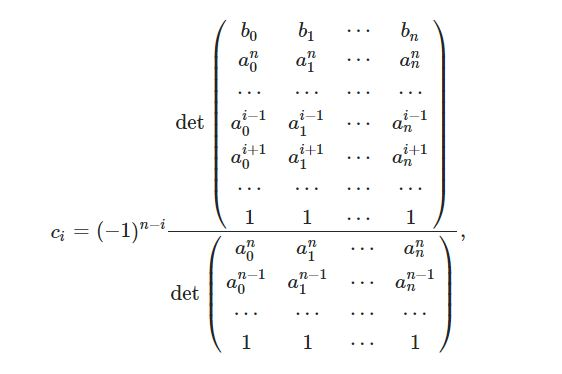
\includegraphics[width=6in, height=3in]{formula.JPG}
	\caption[Optional caption]{}
	\label{}
\end{figure} 
\cleardoublepage
\section{Test Result} 
A simple test result with given example file is following;
\begin{figure}[H]
    \centering
	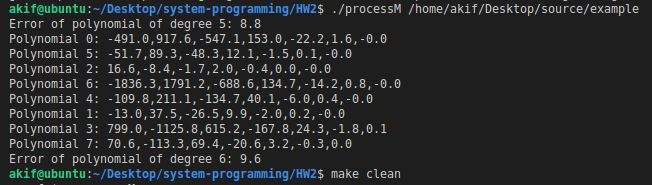
\includegraphics[width=6in, height=3in]{result.JPG}
	\caption[Optional caption]{}
	\label{}
\end{figure}                              
\section{References that was used} 
While doing this howemork following references was used;
\begin{itemize}
	\item Course Textbook Listing 26-5: Reaping dead children via a handler for SIGCHLD
	\item Lagrange’s Interpolation
	\item Determinant Operation
\end{itemize}
\textbf{Note:}Homework was finished as expected. Only problem in 1st round to make error calculation
7th coordinate was used \textbf{not last one}.
\end{document}